%!TEX program = xelatex
\documentclass[a4paper,12pt]{article}
	\linespread{1.3}

\usepackage{geometry} 
	\geometry{left=3cm}
	\geometry{right=1cm}
	\geometry{top=2cm}
	\geometry{bottom=2cm}

\usepackage[fleqn]{amsmath}
\usepackage{unicode-math}
\usepackage{multirow}

\usepackage[english,russian]{babel}
\usepackage{indentfirst}

\usepackage{graphicx}
	\let\ORIincludegraphics\includegraphics
	%\renewcommand{\includegraphics}[2][]{\ORIincludegraphics[scale=0.7,#1]{#2}}

\usepackage{fontspec}
	\defaultfontfeatures{Scale=MatchLowercase}
	\setmainfont[Mapping=tex-text]{Minion Pro}
	\setmonofont{Menlo}

\usepackage{listings}
	\lstset{
		extendedchars=true,
		showspaces=false,
		showtabs=false,
		breaklines=true,
		showstringspaces=false,
		breakatwhitespace=true,
		basicstyle=\ttfamily\small
	}
\usepackage{verbatim}

\usepackage[dvipsnames]{xcolor}

\usepackage{tabularx,booktabs}

\usepackage[nooneline]{caption}
	\captionsetup{textformat=period, figurename=Рисунок}
	\captionsetup[table]{justification=raggedright}
	\captionsetup[figure]{justification=centering} 
	\DeclareCaptionLabelSeparator{tier}{ --- }
	\captionsetup{labelsep=tier}

\usepackage{subcaption}
	\DeclareCaptionSubType*{figure}
	\renewcommand{\thesubfigure}{\asbuk{subfigure}}

\usepackage{floatrow}
	\floatsetup[table]{capposition=top}

\usepackage{pdflscape}
\usepackage{calc}
\usepackage{enumitem}
\makeatletter
    \AddEnumerateCounter{\asbuk}{\@asbuk}{м)}
	\makeatother
	\setlist{nolistsep}
	\renewcommand{\labelitemi}{--}
	\renewcommand{\labelitemii}{--}
	\renewcommand{\labelitemiii}{--}
	\renewcommand{\labelenumi}{\asbuk{enumi})}
	\renewcommand{\labelenumii}{\arabic{enumii})}
	\renewcommand{\labelenumiii}{\asbuk{enumiii})}

\usepackage{tikz}
	\usetikzlibrary{arrows}

\usepackage{titlesec}
	\titleformat{\chapter}[display]
	    {\filcenter}
	    {}
	    {8pt}
	    {\bfseries}{}

	\titleformat{\section}
	    {\normalsize\bfseries}
	    {\thesection}
	    {1em}{}
 
	\titleformat{\subsection}
	    {\normalsize\bfseries}
	    {\thesubsection}
	    {1em}{}

    \titlespacing*{\chapter}{0pt}{-30pt}{8pt}
	\titlespacing*{\section}{\parindent}{*4}{*4}
	\titlespacing*{\subsection}{\parindent}{*4}{*4}
	\titlespacing*{\subsubsection}{\parindent}{*4}{*4}

\usepackage{tocloft}
	\renewcommand{\cfttoctitlefont}{\hspace{0.38\textwidth} \bfseries\MakeUppercase}

\usepackage{titletoc}
	\dottedcontents{section}[1em]{}{1em}{1pc}

\addto\captionsrussian{% Replace "english" with the language you use
  \renewcommand{\contentsname}%
    {СОДЕРЖАНИЕ}%
}


\newcommand*\oline[1]{%
  \vbox{%
    \hrule height 0.5pt%                  % Line above with certain width
    \kern0.25ex%                          % Distance between line and content
    \hbox{%
      \kern-0.1em%                        % Distance between content and left side of box, negative values for lines shorter than content
      \ifmmode#1\else\ensuremath{#1}\fi%  % The content, typeset in dependence of mode
      \kern-0.1em%                        % Distance between content and left side of box, negative values for lines shorter than content
    }% end of hbox
  }% end of vbox
}

%\usepackage{array}
%\newcolumntype{x}[1]{>{\centering\let\newline\\\arraybackslash\hspace{0pt}}p{#1}}

\input{kvmacros}
\begin{document}
	%%!TEX root = main.tex
\begin{titlepage}

\begin{center}
  Министерство образования и науки РФ \\
  Рязанский Государственный Радиотехнический Университет \\
  \vspace{0.2cm}
  Кафедра \\
  \vspace{18em}
  \Large Отчёт по лабораторной работе N  \\
  \textbf{<<>>} 
\end{center}

\vspace{14em}

\begin{flushright}
  Выполнили: \\ студент группы 041 Володин А. Д. \\
                студент группы 041 Силкин Д. В. \\
  \vspace{1.5em}
  Проверили: \\ 
             \\ 
\end{flushright}

\vspace{\fill}

\begin{center}
  Рязань 2013
\end{center}

\end{titlepage}
	\setcounter{page}{2}
	\tableofcontents
	\newpage
	%!TEX root = main.tex

\begin{center}
\textbf{ВВЕДЕНИЕ}
\end{center}
\addcontentsline{toc}{section}{ВВЕДЕНИЕ}

Теория автоматов --- самостоятельный раздел математики, имеющий разнообразную проблематику и приложения.  Основными понятиями теории автоматов являются понятия абстрактного автомата и понятие композиции автоматов. Эти понятия являются разумными абстракциями реально существующих дискретных устройств --- автоматов. Понятие абстрактного автомата позволяет характеризовать устройство с точки зрения алгоритма его функционирования, т.е. алгоритма переработки информации, который оно реализует. Понятие композиции автоматов позволяет характеризовать устройство с точки зрения его структуры, иными словами, даёт представление, каким образом данное устройство построено из других, более элементарных.

Академик В.М. Глушков показал, что любое устройство обработки цифровой информации можно представить в виде совокупности двух взаимодействующих автоматов --- управляющего УА и операционного ОА (Рисунок \ref{figure:intro_pic}).

\begin{figure}[H]
	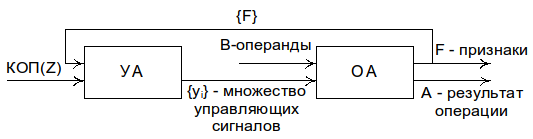
\includegraphics[scale=0.6]{images/intro.png}
	\caption{Структура цифрового автомата}
	\label{figure:intro_pic}
\end{figure}

ОА осуществляет непосредственную обработку данных путем выполнения элементарных операций над словами и выдает результат преобразования в виде двух слов: $A$ (результат) и $F$ (признаки результата, т.е. сигналы о знаках и особых значениях промежуточных и конечных результатов операций). Выполнение элементарных операций инициируется соответствующими управляющими сигналами {$y_0, y_1, y_2 ... y_m$}, которые формируются УА. 

В курсовой работе требуется разработать ОА, реализующий заданный набор арифметико-логических операций.

	%!TEX root = main.tex

\newpage
\section{Задание}

Синтезировать 4-разрядный ОА, реализующий две операции --- арифметическую и логическую, в соответствии с заданным вариантом (Таблица \ref{table:task}). Работу ОА промоделировать, используя САПР <<Альтера>> Max+plus II.

\begin{table}[H]
	\centering
	\caption{Операции, реализуемые ОА}
	\label{table:task}
	\begin{tabular}{| l | l | l | p{2.2cm} | p{2.2cm} | c | c | c | c | c |} \hline
		\multirow{2}{2cm}{Вариант} & \multirow{2}{2cm}{Операция} & \multirow{2}{2cm}{Код} & \multirow{2}{2.2cm}{Элементы памяти ОА1} & \multirow{2}{2.2cm}{Элементы памяти ОА2} & \multicolumn{5}{c|}{Признаки} \\ \cline{6-10}
		& & & & & S & Z & C' & P & C \\ \hline 
		\multirow{2}{2cm}{2в, 1} & $A \leftarrow A - 1$ & 8421+3 & JK & \multirow{2}{2.2cm}{DC} & + & + & + & + & - \\ \cline{2-4} \cline{6-10}

		& $A \leftarrow A \& B$ & двоичный & JK & & + & + & 0 & + & 0 \\ \hline 
	\end{tabular}
\end{table}


\newpage
\section{Структура ОА}

На этапе структурного синтеза ОА представляют в виде двух частей --- памяти и комбинационной схемы КС (Рисунок \ref{figure:oooa}). КС служит для преобразования входных сигналов Х и информации о состоянии устройства (А) в выходные сигналы Y и сигналы возбуждения элементов памяти U.

\begin{figure}[H]
	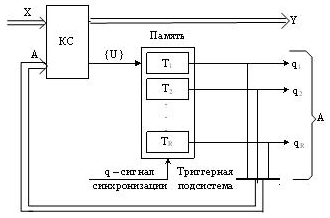
\includegraphics[scale=0.6]{images/2.png}
	\caption{Обобщенная структура ОА}
	\label{figure:oooa}
\end{figure}

Поведение структуры (Рисунок \ref{figure:oooa}) описывается четырьмя группами различных сигналов:

$X$ --- входное слово,

$Y = (X,A)$ --- выходное слово,

$U = \psi(X,A)$ --- слово (функция), обеспечивающее порядок смены состояний автомата

$A$ --- слово, характеризующее состояние автомата.

Внутреннее состояние автомата $А$ определяется состоянием триггеров $a_r \in \{0, 1\}$  и описывается словом состояния $A = (a_1, a_2, a_3, ..., a_i, ... a_r), r = \oline{1,R}$. Множество слов $A$ определяет объем памяти ОА.

Синтезируемый ОА является 4-х разрядным и формирует слово состояния $A = a_3a_2a_1a_0$ .


\newpage
\section{Синтез ОА}

Задача синтеза ОА сводится к:
\begin{itemize}
	\item выбору типа элементов памяти (триггеров), который задан заранее (в данной курсовой работе --- JK-триггеры);
	\item разработке КС, для чего необходимо сформировать систему переключательных функций, описывающую ее поведение:

	$\begin{cases}
			U = \psi(X, A), \\ Y = \lambda(X, A)
	\end{cases}$ (1)
	\item реализации системы ПФ (1) на заданной элементной базе (в данной курсовой работе используется элементная база САПР <<Альтера>> Max+plus II).

\end{itemize}

В случае, если автомат оказывается сложным, задачу синтеза ОА упрощают, декомпозируя (разделяя) его на более простые автоматы ОА$_1$ и ОА$_2$ (Рисунок \ref{figure:decomp}) с одинаковой структурой (Рисунок \ref{figure:srtuct}).

\begin{figure}[H]
	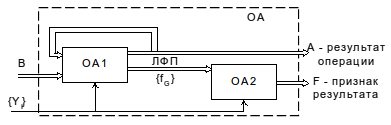
\includegraphics[scale=0.6]{images/3.png}
	\caption{Декомпозиция ОА}
	\label{figure:decomp}
\end{figure}

\begin{figure}[H]
	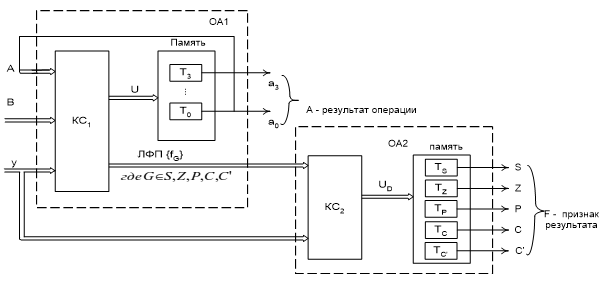
\includegraphics[scale=0.6]{images/4.png}
	\caption{Структурное представление ОА1 и ОА2}
	\label{figure:srtuct}
\end{figure}

Арифметико-логический автомат ОА$_1$ формирует слово результата операции $А$ и сигналы $f_S$, $f_Z$, $f_C'$, $f_P$, $f_C$ --- логические функции признаков (ЛФП), относящиеся к выходным сигналам $Y=\lambda(X, A)$, на основе которых ОА$_2$ формирует уже сами признаки --- слово $F = (S, Z, P, C, C')$ в соответствии с логикой признаков, которая задается таблично (Таблица \ref{table:task}) для каждой отдельной операции.

Операции, реализуемые ОА (Рисунок \ref{figure:decomp}), инициализируются управляющими сигналами $yi$. В данной работе используется только один управляющий сигнал $y$. Если этот сигнал принимает значение $0$, то выполняется арифметическая операция, иначе --- логическая.

\subsection{Синтез ОА${}_1$}


ОА$_1$ можно рассматривать как многооперационный автомат, способный реализовать не одну, а несколько операций. Синтез автомата ОА$_1$ разделяется на синтез автоматов ОА$^{(0)}_{1}$ и ОА$^{(1)}_{1}$ с памятью на  JK-триггерах, реализующих соответственно: 

\begin{itemize}
	\item операцию декремента $A \leftarrow A-1$ в коде 8421+3, инициируемую сигналом $y_0$.
	\item операцию логического умножения $A \leftarrow A \& B$ , инициируемую сигналом $y_1$.

\end{itemize}

Абстрактное представление ОА$_1$ изображено на рисунке \ref{figure:abs_oa1}.

\begin{figure}[H]
	\begin{subfigure}[b]{0.3\textwidth}
		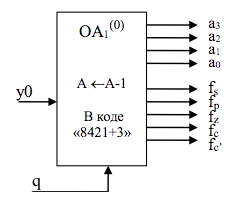
\includegraphics[scale=0.7]{images/abs10.png}
	\end{subfigure}
	\qquad
	\begin{subfigure}[b]{0.3\textwidth}
		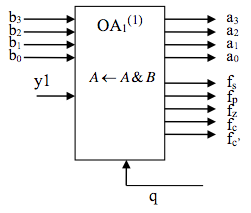
\includegraphics[scale=0.7]{images/abs11.png}
	\end{subfigure}
	\caption{Абстрактное представление ОА1}
	\label{figure:abs_oa1}
\end{figure}

ОА$^{(0)}_{1}$ реализует операцию над одним словом $А$ с установкой результата, поэтому ОА не декомпозируется, и синтезируется как единый 4-х разрядный ОЭ.

ОА$^{(1)}_{1}$ реализует операцию над двумя 4-х разрядными словами $А$ и $В$ с установкой результата. Сигналы возбуждения и выходов являются функциями восьми аргументов. При рассмотрении такого автомата как единого ОЭ синтез значительно усложнится (КТ будет содержать $256 = 2^8$ наборов), поэтому ОА$^{(1)}_{1}$ декомпозируется и синтезируется как композиция одноразрядных ОЭ.


\subsubsection{Синтез ОА$^{(0)}_{1}$}

Автомат ОА$^{(0)}_{1}$ описывается функциями переходов $A(t+1) = \delta^0(A(t))=\delta^0(a_3,a_2,a_1,a_0)$ и выходов $f^0_{G} = f^0_{G}(A(t)) = f^0_{G}(a_3,a_2,a_1,a_0)$, $G = S, Z, C', P, C$, которые  определяют структуру совмещенной кодированной таблицы (Таблица 2). Каждому значению $A(t)$ ставится в соответствие двоичный вектор следующего состояния автомата $A(t+1) = a^*_3,a^*_2,a^*_1,a^*_0$ как результат функции перехода $\delta^0$ операции $y_0: (A \leftarrow A-1)$.

\begin{landscape}
\begin{table}[H]
	\centering
	\caption{Совмещенная КТ для ОА$^{(0)}_{1}$}
	\label{table:OA10f}
	\begin{tabular}{|l|*{22}{c|}{r|}} \hline
		\multirow{3}{0.5cm}{N}
		& \multicolumn{4}{p{2cm}|}{Текущее состояние ОА$^{(0)}_{1}$}
		& \multicolumn{4}{p{2cm}|}{Следующее состояние ОА$^{(0)}_{1}$}
		& \multicolumn{8}{c|}{ФВ $T^0_j$}
		& \multicolumn{5}{c|}{\multirow{2}{2cm}{ЛФП}} \\ \cline{2-17}

		& \multicolumn{4}{c|}{$A(t)$}
		& \multicolumn{4}{c|}{$A(t+1)$}
		& \multicolumn{2}{c|}{$T_3$} 
		& \multicolumn{2}{c|}{$T_2$} 
		& \multicolumn{2}{c|}{$T_1$} 
		& \multicolumn{2}{c|}{$T_0$}
		& \multicolumn{5}{c|}{} \\  \cline{2-22}

		& $a_3$ & $a_2$ & $a_1$ & $a_0$
		& $a^*_3$ & $a^*_2$ & $a^*_1$ & $a^*_0$
		& $J^{(0)}_{3}$ & $K^{(0)}_{3}$ & $J^{(0)}_{2}$ & $K^{(0)}_{2}$  
		& $J^{(0)}_{1}$ & $K^{(0)}_{1}$ & $J^{(0)}_{0}$ & $K^{(0)}_{0}$
		& $f^{(0)}_{S}$ & $f^{(0)}_{Z}$ & $f^{(0)}_{C'}$ & $f^{(0)}_{P}$ & $f^{(0)}_{C}$ \\ \hline

0 & 	0 & 0 & 1 & 1 & 	1 & 1 & 0 & 0 & 	1 & x & 1 & x & x & 1 & x & 1 & 	1 & 0 & 0 & 1 & 0 \\ \hline
1 & 	1 & 1 & 0 & 0 & 	1 & 0 & 1 & 1 & 	x & 0 & x & 1 & 1 & x & 1 & x & 	1 & 0 & 1 & 0 & 0 \\ \hline
2 & 	1 & 0 & 1 & 1 & 	1 & 0 & 1 & 0 & 	x & 0 & 0 & x & x & 0 & x & 1 & 	1 & 0 & 0 & 1 & 0 \\ \hline
3 & 	1 & 0 & 1 & 0 & 	1 & 0 & 0 & 1 & 	x & 0 & 0 & x & x & 1 & 1 & x & 	1 & 0 & 0 & 1 & 0 \\ \hline
4 & 	1 & 0 & 0 & 1 & 	1 & 0 & 0 & 0 & 	x & 0 & 0 & x & 0 & x & x & 1 & 	1 & 0 & 0 & 0 & 0 \\ \hline
5 & 	1 & 0 & 0 & 0 & 	0 & 1 & 1 & 1 & 	x & 1 & 1 & x & 1 & x & 1 & x & 	0 & 0 & 1 & 0 & 0 \\ \hline
6 & 	0 & 1 & 1 & 1 & 	0 & 1 & 1 & 0 & 	0 & x & x & 0 & x & 0 & x & 1 & 	0 & 0 & 0 & 1 & 0 \\ \hline
7 & 	0 & 1 & 1 & 0 & 	0 & 1 & 0 & 1 & 	0 & x & x & 0 & x & 1 & 1 & x & 	0 & 0 & 0 & 1 & 0 \\ \hline
8 & 	0 & 1 & 0 & 1 & 	0 & 1 & 0 & 0 & 	0 & x & x & 0 & 0 & x & x & 1 & 	0 & 0 & 0 & 0 & 0 \\ \hline
9 & 	0 & 1 & 0 & 0 & 	0 & 0 & 1 & 1 & 	0 & x & x & 1 & 1 & x & 1 & x & 	0 & 1 & 1 & 1 & 0 \\ \hline
		

	\end{tabular}
\end{table}
\end{landscape}

Для каждого из триггеров $T_3 \div T_0$ на основе смены их состояний $a_i \rightarrow a^{*}_i, i=\oline{0,3}$ в соответствии с матрицей переходов (таблица \ref{table:JK_SMW}) формируются двоичные сигналы функций возбуждения (ФВ) $T^0_j, j=\oline{0,3}$, под действием которых они меняют свои состояния. В соответствии с таблицей \ref{table:OA10f} при выполнении операции со словом $A$ устанавливаются логические функции признаков (ЛФП) $f_S$, $f_Z$, $f_P$, $f_C'$. Признак $f_C$ остаётся неизменным.

Признаки:
\begin{itemize}
	\item fS --- фиксирует знаковый бит результата,
	\item fZ --- фиксирует нулевой результат,
	\item fP --- фиксирует четное число единиц результата,
	\item fC --- фиксирует перенос (заем) из старшего бита результата,
	\item fC’---  фиксирует вспомогательный перенос (заем) из бита $а_2$ результата.
\end{itemize}

\begin{table}[H]
	\centering
	\caption{Матрица переходов JK-триггера}
	\label{table:JK_SMW}
	\begin{tabular}{| l | p{1cm} | p{1cm} |} \hline
		\multirow{2}{*}{Переход} & \multicolumn{2}{c|}{Вход триггера}\\ \cline{2-3}
		& J & K \\ \hline
		$0 \rightarrow 0$ & 	$0$ & $x$ \\ \hline
		$0 \rightarrow 1$ & 	$1$ & $x$ \\ \hline
		$1 \rightarrow 0$ & 	$x$ & $1$ \\ \hline
		$1 \rightarrow 1$ & 	$x$ & $0$ \\ \hline
	\end{tabular}
\end{table}

Полученные функции  $J^{(0)}_{3}$, $K^{(0)}_{3}$, $J^{(0)}_{2}$, $K^{(0)}_{2}$, $J^{(0)}_{1}$, $K^{(0)}_{1}$, $J^{(0)}_{0}$, $K^{(0)}_{0}$, $f^{(0)}_{S}$, $f^{(0)}_{Z}$, $f^{(0)}_{C'}$, $f^{(0)}_{P}$, $f^{(0)}_{C}$  заносятся на карты Карно для минимизации (Рисунок \ref{figure:oa10_min_trig}, \ref{figure:oa10_min_flags}).

%!TEX root = main.tex
\kvnoindex
\begin{figure}[H]
	\begin{subfigure}[b]{0.3\textwidth}
	\karnaughmap{4}%
	{$J^{(0)}_3:$}%
	{{$a_1$}{$a_3$}{$a_0$}{$a_2$}}%
	{x0x0xxxxx010xxxx}%
	{%
		\textcolor{Blue}{%
			\put(4, 2){\oval(1.9, 3.9)[l]}
			\put(0, 2){\oval(1.9, 3.9)[r]}
		}%
	}
	\caption{}
	\label{figure:oa10_min_J3}
	\end{subfigure}
	\qquad
	\begin{subfigure}[b]{0.3\textwidth}
	\karnaughmap{4}%
	{$K^{(0)}_3:$}%
	{{$a_1$}{$a_3$}{$a_0$}{$a_2$}}%
	{xxxx100xxxxx0x0x}%
	{%
		\textcolor{Blue}{%
			\put(4, 3.5){\oval(1.9, 0.9)[l]}
			\put(0, 3.5){\oval(1.9, 0.9)[r]}
		}%
	}
	\caption{}
	\label{figure:oa10_min_K3}
	\end{subfigure}

	\begin{subfigure}[b]{0.3\textwidth}
	\karnaughmap{4}%
	{$J^{(0)}_2:$}%
	{{$a_1$}{$a_3$}{$a_0$}{$a_2$}}%
	{xxxx1x0xxx1x0x0x}%
	{%
		\textcolor{Blue}{%
			\put(2, 3.5){\oval(3.9, 0.9)[l]}
			\put(2, 3.5){\oval(3.9, 0.9)[r]}
		}%
		\textcolor{Red}{%
			\put(1, 2){\oval(1.9, 3.9)[t]}
			\put(1, 2){\oval(1.9, 3.9)[b]}
		}%
	}
	\caption{}
	\label{figure:oa10_min_J2}
	\end{subfigure}
	\qquad
	\begin{subfigure}[b]{0.3\textwidth}
	\karnaughmap{4}%
	{$K^{(0)}_2:$}%
	{{$a_1$}{$a_3$}{$a_0$}{$a_2$}}%
	{x1x0x1xxx0x0xxxx}%
	{%
		\textcolor{Blue}{%
			\put(2, 3.5){\oval(3.9, 0.9)[l]}
			\put(2, 3.5){\oval(3.9, 0.9)[r]}
		}%
	}
	\caption{}
	\label{figure:oa10_min_K2}
	\end{subfigure}	

	\begin{subfigure}[b]{0.3\textwidth}
	\karnaughmap{4}%
	{$J^{(0)}_1:$}%
	{{$a_1$}{$a_3$}{$a_0$}{$a_2$}}%
	{x1x0110xxxxxxxxx}%
	{%
		\textcolor{Blue}{%
			\put(2, 0){\oval(3.9, 1.9)[t]}
			\put(2, 4){\oval(3.9, 1.9)[b]}
		}%
	}
	\caption{}
	\label{figure:oa10_min_J1}
	\end{subfigure}
	\qquad
	\begin{subfigure}[b]{0.3\textwidth}
	\karnaughmap{4}%
	{$K^{(0)}_1:$}%
	{{$a_1$}{$a_3$}{$a_0$}{$a_2$}}%
	{xxxxxxxxx1101x0x}%
	{%
		\textcolor{Blue}{%
			\put(2, 0){\oval(3.9, 1.9)[t]}
			\put(2, 4){\oval(3.9, 1.9)[b]}
		}%
		\textcolor{Red}{%
			\put(0.5, 2){\oval(0.9, 3.9)[t]}
			\put(0.5, 2){\oval(0.9, 3.9)[b]}
		}%
	}
	\caption{}
	\label{figure:oa10_min_K1}
	\end{subfigure}

	\begin{subfigure}[b]{0.3\textwidth}
	\karnaughmap{4}%
	{$J^{(0)}_0:$}%
	{{$a_1$}{$a_3$}{$a_0$}{$a_2$}}%
	{x1xx11xxx1xx1xxx}%
	{%
		\textcolor{Blue}{%
			\put(2, 2){\oval(3.9, 3.9)[l]}
			\put(2, 2){\oval(3.9, 3.9)[r]}
		}%
	}
	\caption{}
	\label{figure:oa10_min_J0}
	\end{subfigure}
	\qquad
	\begin{subfigure}[b]{0.3\textwidth}
	\karnaughmap{4}%
	{$K^{(0)}_0:$}%
	{{$a_1$}{$a_3$}{$a_0$}{$a_2$}}%
	{xxx1xx1xxx11xx1x}%
	{%
	{%
		\textcolor{Blue}{%
			\put(2, 2){\oval(3.9, 3.9)[l]}
			\put(2, 2){\oval(3.9, 3.9)[r]}
		}%
	}	
	}
	\caption{}
	\label{figure:oa10_min_K0}
	\end{subfigure}	
	
	\caption{Карты Карно для ФВ ОА$^{(0)}_{1}$}
	\label{figure:oa10_min_trig}
\end{figure}

\begin{figure}[H]
	\begin{subfigure}[b]{0.3\textwidth}
	\karnaughmap{4}%
	{$f^{(0)}_s:$}%
	{{$a_1$}{$a_3$}{$a_0$}{$a_2$}}%
	{x0x0011xx0101x1x}%
	{%
		{%
		\textcolor{Blue}{%
			\put(4, 1){\oval(1.9, 1.9)[l]}
			\put(0, 1){\oval(1.9, 1.9)[r]}
		}%
		\textcolor{Red}{%
			\put(3, 2){\oval(1.9, 1.9)[l]}
			\put(3, 2){\oval(1.9, 1.9)[r]}
		}%
		\textcolor{Green}{%
			\put(2.5, 2){\oval(0.9, 3.9)[t]}
			\put(2.5, 2){\oval(0.9, 3.9)[b]}
		}%
	}
	}
	\caption{}
	\label{figure:oa10_min_fs}
	\end{subfigure}
	\qquad
	\begin{subfigure}[b]{0.3\textwidth}
	\karnaughmap{4}%
	{$f^{(0)}_z:$}%
	{{$a_1$}{$a_3$}{$a_0$}{$a_2$}}%
	{x1x0000xx0000x0x}%
	{%
		{%
		\textcolor{Blue}{%
			\put(1, 3.5){\oval(1.9, 0.9)[l]}
			\put(1, 3.5){\oval(1.9, 0.9)[r]}
		}%
		}
	}
	\caption{}
	\label{figure:oa10_min_fz}
	\end{subfigure}

	\begin{subfigure}[b]{0.3\textwidth}
	\karnaughmap{4}%
	{$f_c:$}%
	{{$a_1$}{$a_3$}{$a_0$}{$a_2$}}%
	{x0x0000xx0100x0x}%
	{%
	\textcolor{Blue}{%
			\put(0.5, 2){\oval(0.9, 3.9)[t]}
			\put(0.5, 2){\oval(0.9, 3.9)[b]}
		}%
	}
	\caption{}
	\label{figure:oa10_min_fc}
	\end{subfigure}
	\qquad
	\begin{subfigure}[b]{0.3\textwidth}
	\karnaughmap{4}%
	{$f^{(0)}_p:$}%
	{{$a_1$}{$a_3$}{$a_0$}{$a_2$}}%
	{x1x0000xx1111x1x}%
	{%
		{%
		\textcolor{Blue}{%
			\put(2, 1){\oval(3.9, 1.9)[l]}
			\put(2, 1){\oval(3.9, 1.9)[r]}
		}%
		\textcolor{Red}{%
			\put(1, 0){\oval(1.9, 1.9)[t]}
			\put(1, 4){\oval(1.9, 1.9)[b]}
		}%
	}
	}
	\caption{}
	\label{figure:oa10_min_fp}
	\end{subfigure}	
	
	\begin{subfigure}[b]{0.3\textwidth}
	\karnaughmap{4}%
	{$f^{(0)}_{c'}:$}%
	{{$a_1$}{$a_3$}{$a_0$}{$a_2$}}%
	{x100110xx0x00x0x}%
	{%
		{%
		\textcolor{Blue}{%
			\put(2, 3.5){\oval(3.9, 0.9)[l]}
			\put(2, 3.5){\oval(3.9, 0.9)[r]}
		}%
	}
	}
	\caption{}
	\label{figure:oa10_min_fc1}
	\end{subfigure}

	\caption{Карты Карно для ЛФП ОА$^{(0)}_{1}$}
	\label{figure:oa10_min_flags}
\end{figure}

В результате минимизации получается система ПФ, представленных в МДНФ:

$J^{(0)}_{3} = \oline{a_2}$

$K^{(0)}_{3} = \oline{a_2} \cdot \oline{a_1} \cdot \oline{a_0}$

$J^{(0)}_{2} = \oline{a_3} \vee \oline{a_1} \cdot \oline{a_0}$

$K^{(0)}_{2} = \oline{a_1} \cdot \oline{a_0}$

$J^{(0)}_{1} = \oline{a_0}$

$K^{(0)}_{1} = \oline{a_0} \vee \oline{a_3} \cdot \oline{a_2}$

$J^{(0)}_{0} = 1$

$K^{(0)}_{0} = 1$

$f^{(0)}_{S} = a_3 \cdot a_2 \vee \oline{a_2} \cdot a_1 \vee a_3 \cdot a_0 $

$f^{(0)}_{Z} = \oline{a_3} \cdot \oline{a_1} \cdot \oline{a_0}$

$f^{(0)}_{C'} = \oline{a_1} \cdot \oline{a_0}$

$f^{(0)}_{P} = a_1 \vee \oline{a_3} \cdot \oline{a_0}$

$f^{(0)}_{C} = 0$


\subsubsection{Синтез ОА$^{(1)}_{1}$}

%!TEX root = main.tex

\begin{figure}[H]
\begin{subfigure}[b]{0.3\textwidth}

	\karnaughmap{2}%
	{$J_i:$}%
	{{$b$}{$a$}}%
	{0x0x}%
	{%
	}
	\caption{}
	\label{oa11_J}
\end{subfigure}
\begin{subfigure}[b]{0.3\textwidth}
	\karnaughmap{2}%
	{$K_i:$}%
	{{$b$}{$a$}}%
	{x1x0}%
	{%
	\textcolor{Blue}{
		\put(1,1.5){\oval(1.9,0.9)[]}}
	}
	\caption{}
	\label{oa11_K}
\end{subfigure}
	\caption{oa11mintrig}
	\label{figure:oa11_min_trig}
\end{figure}


\begin{figure}[H]
	\begin{subfigure}[b]{0.3\textwidth}
	\karnaughmap{4}%
	{$f_s:$}%
	{{$r_1$}{$r_3$}{$r_0$}{$r_2$}}%
	{0000111100001111}%
	{%
		\textcolor{Blue}{%
			\put(3, 2){\oval(1.9, 3.9)[t]}
			\put(3, 2){\oval(1.9, 3.9)[b]}
		}%
	}
	\caption{}
	\label{figure:oa11_min_fs}
	\end{subfigure}
	\qquad
	\begin{subfigure}[b]{0.3\textwidth}
	\karnaughmap{4}%
	{$f_z:$}%
	{{$r_1$}{$r_3$}{$r_0$}{$r_2$}}%
	{1000000000000000}%
	{%
		\textcolor{Blue}{
			\put(0.5,3.5){\oval(0.9,0.9)[]}%
		}%	
	}
	\caption{}
	\label{figure:oa11_min_fz}
	\end{subfigure}

	\begin{subfigure}[b]{0.3\textwidth}
	\karnaughmap{4}%
	{$f_p:$}%
	{{$r_1$}{$r_3$}{$r_0$}{$r_2$}}%
	{1001011001101001}%
	{%
		\textcolor{Blue}{
			\put(0.5,3.5){\oval(0.9,0.9)[]}%
			\put(2.5,3.5){\oval(0.9,0.9)[]}%
			\put(1.5,2.5){\oval(0.9,0.9)[]}%
			\put(3.5,2.5){\oval(0.9,0.9)[]}%
			\put(0.5,1.5){\oval(0.9,0.9)[]}%
			\put(2.5,1.5){\oval(0.9,0.9)[]}%
			\put(1.5,0.5){\oval(0.9,0.9)[]}%
			\put(3.5,0.5){\oval(0.9,0.9)[]}%
		}%	
	}
	\caption{}
	\label{figure:oa11_min_fp}
	\end{subfigure}

	\begin{subfigure}[b]{0.3\textwidth}
	\karnaughmap{4}%
	{$f_c:$}%
	{{$r_1$}{$r_3$}{$r_0$}{$r_2$}}%
	{0000000000000000}%
	{}
	
	\caption{}
	\label{figure:oa11_min_fc}
	\end{subfigure}
	\qquad
	\begin{subfigure}[b]{0.3\textwidth}
	\karnaughmap{4}%
	{$f'_c:$}%
	{{$r_1$}{$r_3$}{$r_0$}{$r_2$}}%
	{0000000000000000}%
	{}


	\caption{}
	\label{figure:oa11_min_fc1}
	\end{subfigure}


	\caption{oa11minflags}
	\label{figure:oa11_min_flag}

\end{figure}

\subsubsection{Объединенные ФВ И ЛФП ОА${}_1$}

\subsection{Синтез ОА${}_2$}

	%!TEX root = main.tex

\newpage
\section{Реализация ОА}

Для реализации цифрового автомата использовалась САПР <<Альтера>> Max+plus II.

\subsection{Реализация ОА${}_1$}

Схема построена в соответствии с объединёнными функциями возбуждения и ЛФП, полученными в пункте 3.1.3.

Входными сигналами для ОА${}_1$ являются:
\begin{itemize}
	\item сигнал управления \texttt{Y}, который реализован таким образом, что:
		\begin{itemize}
			\item Y = 1, Y0 = 1. ОА реализует арифметическую операцию, 
			\item Y = 0, Y1 = 1. ОА реализует логическую операцию.
		\end{itemize}
	\item операнд \texttt{B} для логической операции,
	\item сигнал синхронизации \texttt{Q},
	\item сигнал \texttt{LDA} для принудительной установки триггеров в заданное состояние,
	\item сигнал \texttt{SETN} разрешения принудительной установки триггеров в заданное состояние.
\end{itemize}

Выходными сигналами для ОА${}_1$ являются:
\begin{itemize}
	\item новое состояние автомата \texttt{A},
	\item ЛФП \texttt{FS}, \texttt{FZ}, \texttt{FC1}, \texttt{FP}, \texttt{FC}.
\end{itemize}

Поскольку после включения питания все триггеры будут находиться в нулевом состоянии, использована схема принудительной установки состояния автомата в заданное.

Для выполнения различных операций используется одна и та же память, то есть одни и те же триггеры, возбуждаемые различными функциями. Поэтому схемы формирования функций возбуждения и ЛФП представлены в виде отдельных символов oa10\textunderscore logic и oa11\textunderscore logic для ОА$^{(0)}_{1}$ и ОА$^{(1)}_{1}$ соответственно.

Так как используются две схемы формирования функций возбуждения и ЛФП, то реализована схема, позволяющая подключить выходы одной из них к входам триггеров в зависимости от кода операции \texttt{Y}.

\begin{figure}[H]
	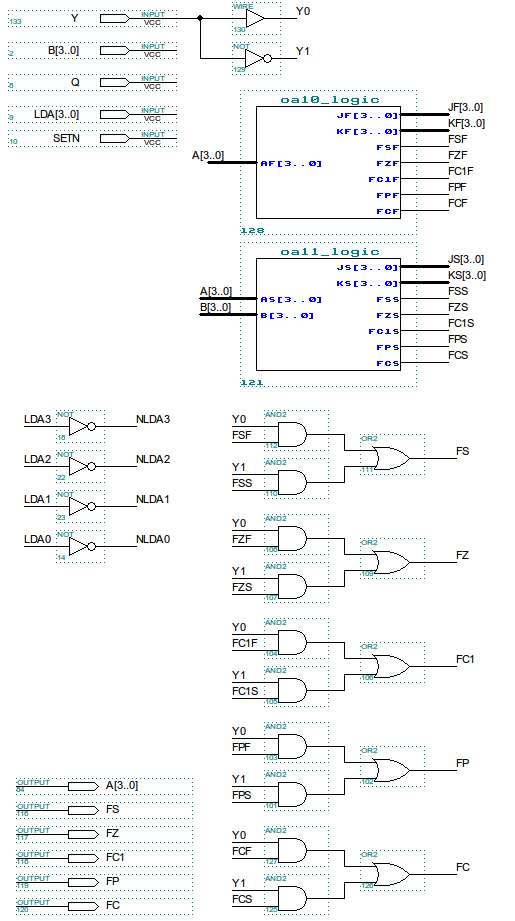
\includegraphics[scale=0.6]{images/altera/rev2/oa1_1_WITH_CONTROL_SIGNAL.png}
	\caption{Cхема ОА$_{1}$ (начало)}
	\label{figure:oa1-1log}
\end{figure}

\begin{figure}[H]
	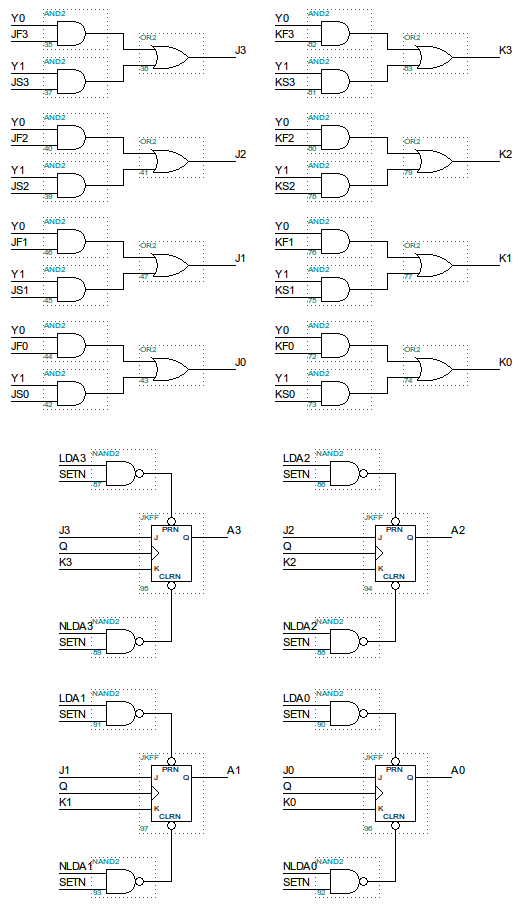
\includegraphics[scale=0.6]{images/altera/rev2/oa1_2.png}
	\caption{Cхема ОА$_{1}$ (окончание)}
	\label{figure:oa1-2log}
\end{figure}

\begin{figure}[H]
	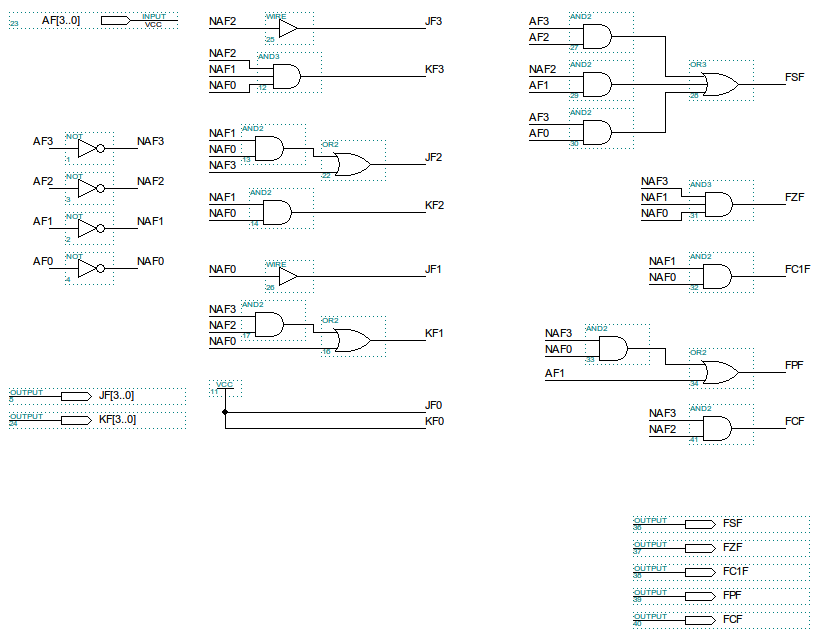
\includegraphics[scale=0.6]{images/altera/rev2/oa10_logic.png}
	\caption{Схема формирования функций возбуждения и ЛФП ОА$^{(0)}_{1}$}
	\label{figure:oa10log}
\end{figure}

\begin{figure}[H]
	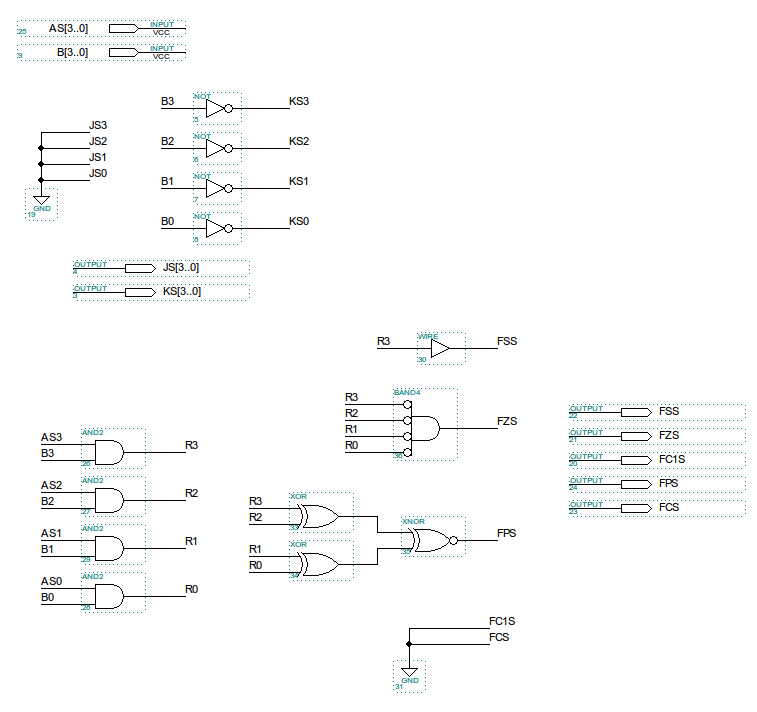
\includegraphics[scale=0.6]{images/altera/rev2/oa11_logic.png}
	\caption{Схема формирования функций возбуждения и ЛФП ОА$^{(1)}_{1}$}
	\label{figure:oa11log}
\end{figure}


\clearpage
\subsection{Реализация ОА${}_2$}

Схема построена в соответствии с объединёнными функциями возбуждения для каждого признака, полученными в пункте 3.2.

Для проверки сохранения значения признака \texttt{C} в соответствии с заданием (Таблица \ref{table:task}) реализован сигнал \texttt{PRNC} принудительной установки признака \texttt{С}. При \texttt{PRNC = 1} автомат устанавливает признак \texttt{C}.

При выполнении логической операции (по сигналу \texttt{Y1}) в соответствии с заданием (Таблица \ref{table:task}) автомат должен устанавливать значения признаков C и C' (на схеме признак С' обозначен как С1) равными нулю. Для этого использован сигнал '0'.

Входными сигналами для ОА${}_2$ являются:
\begin{itemize}
	\item осведомительные сигналы \texttt{FS}, \texttt{FZ}, \texttt{FC1}, \texttt{FP}, \texttt{FC},
	\item сигнал синхронизации \texttt{Q},
	\item сигнал управления \texttt{Y}.
\end{itemize}

Выходными сигналами для ОА${}_2$ являются флаги \texttt{S}, \texttt{Z}, \texttt{C1}, \texttt{P}, \texttt{C}.

\begin{figure}[H]
	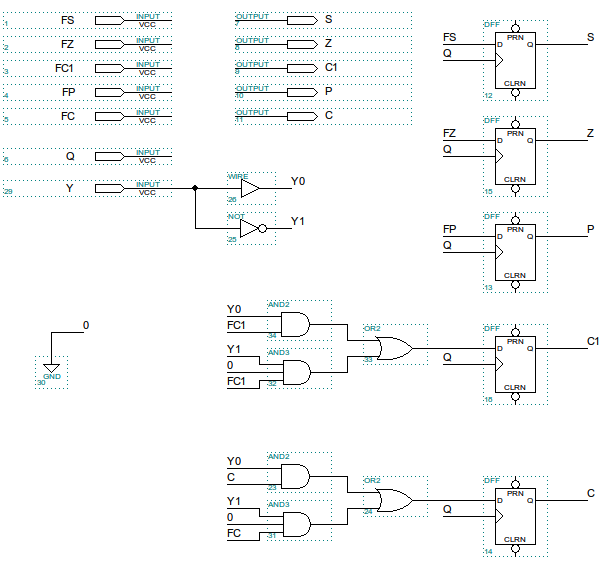
\includegraphics[scale=0.6]{images/altera/rev2/OA2_PRNC/OA2_PRNC_WIDE.png}
	\caption{Cхема ОА$_{2}$}
	\label{figure:oa2log}
\end{figure}

\clearpage
\subsection{Реализация ОА}

Схема операционного автомата (Рисунок \ref{figure:oalog}) представлена в виде совокупности схем ОА${}_1$ и ОА${}_2$, представленных в виде символов.

\begin{figure}[H]
	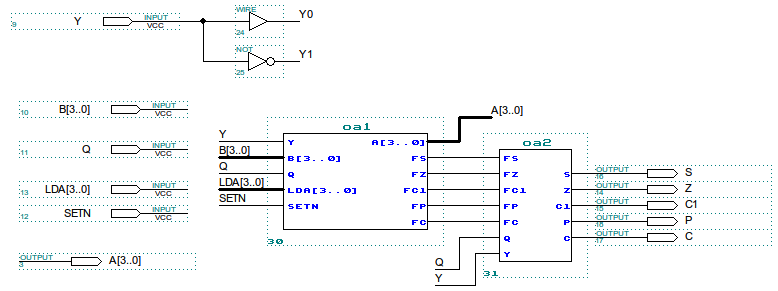
\includegraphics[scale=0.6]{images/altera/rev2/oa_WITH_CONTROL_SIGNAL.png}
	\caption{Cхема ОА}
	\label{figure:oalog}
\end{figure}

\newpage
\section{Моделирование ОА}

\subsection{Методика моделирования}

Процесс моделирования данного автомата был разделен на 3 этапа:
\begin{itemize}
	\item Моделирование ОА$_1$. Целью моделирования ОА1 является проверка правильности выполнении операций, проверка формирования значений логических функций признаков $f_S$, $f_Z$, $f_{C'}$, $f_P$, $f_C$. 
	\item Моделирование ОА$_2$. На данном этапе осуществляется проверка правильности записи значений признаков $S$, $Z$, $C'$, $P$, $C$.
	\item Моделирование ОА. На данном этапе осуществлялась проверка правильности взаимодействия автоматов ОА$_1$ и ОА$_2$. 
\end{itemize}

\subsection{Моделирование ОА$_1$}

\subsubsection{Моделирование арифметической операции}

На вход ОА1 подаются следующие сигналы:
\begin{itemize}
	\item сигнал кода операции \texttt{Y = 1},
	\item сигнал \texttt{LDA = 0011}$_2$, соответствующий числу 3h (первому разрешенному состоянию),
	\item импульс \texttt{SETN}, соответствующий переходу автомата в состояние с шины \texttt{LDA},
	\item импульсы тактовой частоты \texttt{Q}.
\end{itemize}
 
Корректной работе автомата соответствуют значения на выходах, приведенные в таблице \ref{table:oa10test}.

Временная диаграмма результатов моделирования представлена на рисунке \ref{figure:oa10test}.

\clearpage
\begin{table}[H]
	\centering
	\caption{Ожидаемые результаты моделирования операции $A \leftarrow A - 1$}
	\label{table:oa10test}
	\begin{tabular}{|l|*{7}{c|}{r|}} \hline
		A(t) & A(t+1) & FS & FZ & FC1 & FP & FC \\ \hline
		0011 & 1100 & 1 & 0 & 0 & 1 & 1 \\ \hline
		1100 & 1011 & 1 & 0 & 1 & 0 & 0 \\ \hline
		1011 & 1010 & 1 & 0 & 0 & 1 & 0 \\ \hline
		1010 & 1001 & 1 & 0 & 0 & 1 & 0 \\ \hline
		1001 & 1000 & 1 & 0 & 0 & 0 & 0 \\ \hline
  		1000 & 0111 & 0 & 0 & 1 & 0 & 0 \\ \hline
		0111 & 0110 & 0 & 0 & 0 & 1 & 0 \\ \hline
		0110 & 0101 & 0 & 0 & 0 & 1 & 0 \\ \hline
		0101 & 0100 & 0 & 0 & 0 & 0 & 0 \\ \hline
		0100 & 0011 & 0 & 0 & 1 & 1 & 0 \\ \hline
	\end{tabular}
\end{table}

\begin{figure}[H]
	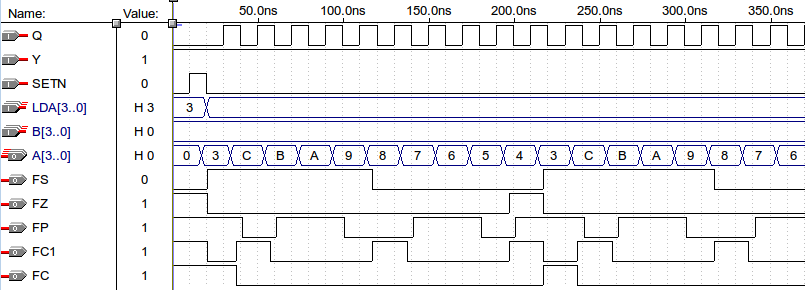
\includegraphics[scale=0.6]{images/altera/rev2/test10.png}
	\caption{Временная диаграмма результатов моделирования операции $A \leftarrow A - 1$}
	\label{figure:oa10test}
\end{figure}

Автомат циклически выполняет заданную операцию $A \leftarrow A - 1$ в коде с избытком 3, вырабатывая сигналы от 3h до Ch в шестнадцатеричной системе счисления. Признаки устанавливаются в соответствии с таблицей \ref{table:oa10test}. То есть автомат функционирует в соответствии с заданием.

\clearpage
\subsubsection{Моделирование логической операции}

На вход ОА1 подаются следующие сигналы:
\begin{itemize}
	\item сигнал кода операции \texttt{Y = 0},
	\item сигналы \texttt{LDA}, соответствующие установке состояния,
	\item импульс \texttt{SETN}, соответствующий переходу автомата в состояние с шины \texttt{LDA},
	\item сигналы \texttt{B},
	\item импульсы тактовой частоты \texttt{Q}.
\end{itemize}
 
Корректной работе автомата соответствуют значения на выходах, приведенные в таблице \ref{table:oa11test}.

Временная диаграмма результатов моделирования представлена на рисунке \ref{figure:oa11test}.

\begin{table}[H]
	\centering
	\caption{Ожидаемые результаты моделирования операции $A \leftarrow A \& B$}
	\label{table:oa11test}
	\begin{tabular}{|l|*{8}{c|}{r|}} \hline
		A(t) & B(t) & A(t+1) & FS & FZ & FC1 & FP & FC \\ \hline
		1010 & 0111 & 0010   & 0  & 0  & 0   & 0   & 0 \\ \hline
		1111 & 1001 & 1001   & 1  & 0  & 0   & 1   & 0 \\ \hline
		1001 & 0110 & 0000   & 0  & 1  & 0   & 1   & 0 \\ \hline
	\end{tabular}
\end{table}

\begin{figure}[H]
	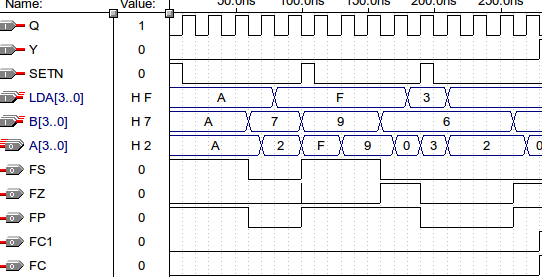
\includegraphics[scale=0.6]{images/ff/11.png}
	\caption{Временная диаграмма результатов моделирования операции $A \leftarrow A \& B$}
	\label{figure:oa11test}
\end{figure}

Из временной диаграммы (Рисунок \ref{figure:oa11test}) видно, что автомат выполняет операцию $A \leftarrow A \& B$ в соответствии с ожидаемыми результатами таблицы \ref{table:oa11test}. 

Если с помощью схемы задания состояния записать в $A$ число 1010$_2$, а на шину $B$ подать сигнал, соответствующий числу 0111$_2$, то после прихода следующего импульса синхронизации $A = A \& B = 1010_2 \& 0111_2 = 0010_2$ и т.д. Признаки устанавливаются в соответствии с таблицей \ref{table:oa11test}. То есть автомат функционирует в соответствии с заданием.

\clearpage
\subsection{Моделирование ОА$_2$}

На триггеры Ds, Dz, Dc1, Dp, Dc подаются:
\begin{itemize}
	\item объединенные функции возбуждения \texttt{FZ}, \texttt{FS}, \texttt{FP}, \texttt{FC1}, \texttt{FC},
	\item управляющий сигнал \texttt{Y},
	\item импульсы тактовой частоты \texttt{Q},
	\item сигнал \texttt{PRNC} принудительной установки признака \texttt{С}.
\end{itemize} 

На выходах ОА$_2$ по положительному фронта синхроимпульса \texttt{Q} записываются значения признаков S, Z, C1, P, C в соответствии со значениями ЛФП из таблиц 2, 5.

\begin{figure}[H]
	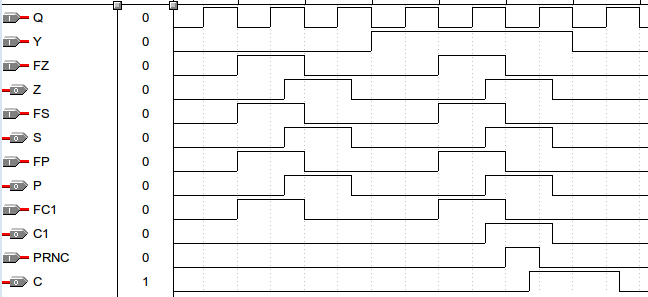
\includegraphics[scale=0.6]{images/ff/2.png}
	\caption{Временная диаграмма результатов моделирования ОА$_2$}
	\label{figure:oa2test}
\end{figure}

Из диаграммы (Рисунок \ref{figure:oa2test}) видно, что схема работает корректно. Значение признака \texttt{C} при выполнении арифметической (Y = 1) операции ОА сохраняет.

\clearpage
\subsection{Моделирование ОА}

На рисунке \ref{figure:oafin0test} приведена временная диаграмма выполнения логической (для Y = 0) и арифметической (для Y = 1) операций, иллюстрирующая работу автомата, состоящего из ОА$_1$ и ОА$_2$.

\begin{figure}[H]
	\begin{subfigure}[b]{1\textwidth}
		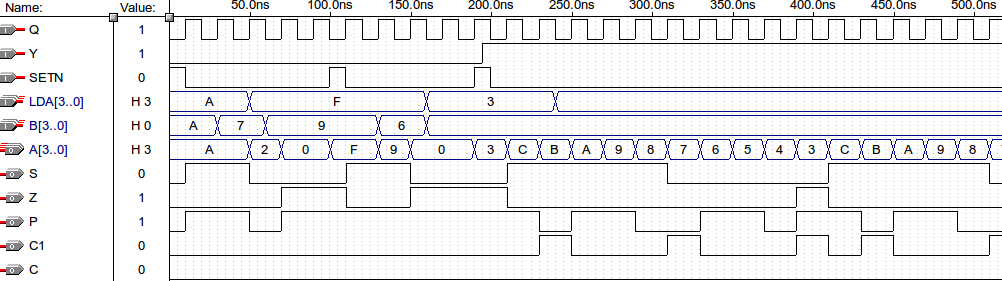
\includegraphics[scale=0.5]{images/ff/001.png}
		\caption{}
	\end{subfigure}
	
	\begin{subfigure}[b]{1\textwidth}
		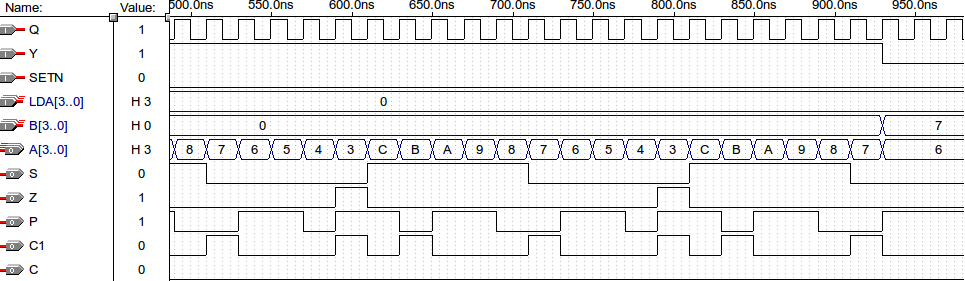
\includegraphics[scale=0.5]{images/ff/002.png}
		\caption{}
	\end{subfigure}
	\caption{Временная диаграмма результатов моделирования ОА}
	\label{figure:oafin0test}
\end{figure}

Из временной диаграммы видно, что результаты выполнения операций и признаки совпадают со значениями из таблиц 2 и 5. Признак \texttt{C}, в соответствии с заданием (Таблица \ref{table:task}), при выполнении арифметической операции ОА не устанавливает.

То есть, автомат функционирует в соответствии с заданием.

	%!TEX root = main.tex

\newpage
%\section*{ЗАКЛЮЧЕНИЕ}
%\addcontentsline{toc}{section}{ЗАКЛЮЧЕНИЕ}
\begin{center}
\textbf{ЗАКЛЮЧЕНИЕ}
\end{center}
\addcontentsline{toc}{section}{ЗАКЛЮЧЕНИЕ}


	%!TEX root = main.tex

\newpage

\begin{center}
\textbf{БИБЛИОГРАФИЧЕСКИЙ СПИСОК}
\end{center}
\addcontentsline{toc}{section}{БИБЛИОГРАФИЧЕСКИЙ СПИСОК}


\end{document}